% Options for packages loaded elsewhere
\PassOptionsToPackage{unicode}{hyperref}
\PassOptionsToPackage{hyphens}{url}
%
\documentclass[
]{article}
\usepackage{amsmath,amssymb}
\usepackage{iftex}
\ifPDFTeX
  \usepackage[T1]{fontenc}
  \usepackage[utf8]{inputenc}
  \usepackage{textcomp} % provide euro and other symbols
\else % if luatex or xetex
  \usepackage{unicode-math} % this also loads fontspec
  \defaultfontfeatures{Scale=MatchLowercase}
  \defaultfontfeatures[\rmfamily]{Ligatures=TeX,Scale=1}
\fi
\usepackage{lmodern}
\ifPDFTeX\else
  % xetex/luatex font selection
\fi
% Use upquote if available, for straight quotes in verbatim environments
\IfFileExists{upquote.sty}{\usepackage{upquote}}{}
\IfFileExists{microtype.sty}{% use microtype if available
  \usepackage[]{microtype}
  \UseMicrotypeSet[protrusion]{basicmath} % disable protrusion for tt fonts
}{}
\makeatletter
\@ifundefined{KOMAClassName}{% if non-KOMA class
  \IfFileExists{parskip.sty}{%
    \usepackage{parskip}
  }{% else
    \setlength{\parindent}{0pt}
    \setlength{\parskip}{6pt plus 2pt minus 1pt}}
}{% if KOMA class
  \KOMAoptions{parskip=half}}
\makeatother
\usepackage{xcolor}
\usepackage[margin=1in]{geometry}
\usepackage{color}
\usepackage{fancyvrb}
\newcommand{\VerbBar}{|}
\newcommand{\VERB}{\Verb[commandchars=\\\{\}]}
\DefineVerbatimEnvironment{Highlighting}{Verbatim}{commandchars=\\\{\}}
% Add ',fontsize=\small' for more characters per line
\usepackage{framed}
\definecolor{shadecolor}{RGB}{248,248,248}
\newenvironment{Shaded}{\begin{snugshade}}{\end{snugshade}}
\newcommand{\AlertTok}[1]{\textcolor[rgb]{0.94,0.16,0.16}{#1}}
\newcommand{\AnnotationTok}[1]{\textcolor[rgb]{0.56,0.35,0.01}{\textbf{\textit{#1}}}}
\newcommand{\AttributeTok}[1]{\textcolor[rgb]{0.13,0.29,0.53}{#1}}
\newcommand{\BaseNTok}[1]{\textcolor[rgb]{0.00,0.00,0.81}{#1}}
\newcommand{\BuiltInTok}[1]{#1}
\newcommand{\CharTok}[1]{\textcolor[rgb]{0.31,0.60,0.02}{#1}}
\newcommand{\CommentTok}[1]{\textcolor[rgb]{0.56,0.35,0.01}{\textit{#1}}}
\newcommand{\CommentVarTok}[1]{\textcolor[rgb]{0.56,0.35,0.01}{\textbf{\textit{#1}}}}
\newcommand{\ConstantTok}[1]{\textcolor[rgb]{0.56,0.35,0.01}{#1}}
\newcommand{\ControlFlowTok}[1]{\textcolor[rgb]{0.13,0.29,0.53}{\textbf{#1}}}
\newcommand{\DataTypeTok}[1]{\textcolor[rgb]{0.13,0.29,0.53}{#1}}
\newcommand{\DecValTok}[1]{\textcolor[rgb]{0.00,0.00,0.81}{#1}}
\newcommand{\DocumentationTok}[1]{\textcolor[rgb]{0.56,0.35,0.01}{\textbf{\textit{#1}}}}
\newcommand{\ErrorTok}[1]{\textcolor[rgb]{0.64,0.00,0.00}{\textbf{#1}}}
\newcommand{\ExtensionTok}[1]{#1}
\newcommand{\FloatTok}[1]{\textcolor[rgb]{0.00,0.00,0.81}{#1}}
\newcommand{\FunctionTok}[1]{\textcolor[rgb]{0.13,0.29,0.53}{\textbf{#1}}}
\newcommand{\ImportTok}[1]{#1}
\newcommand{\InformationTok}[1]{\textcolor[rgb]{0.56,0.35,0.01}{\textbf{\textit{#1}}}}
\newcommand{\KeywordTok}[1]{\textcolor[rgb]{0.13,0.29,0.53}{\textbf{#1}}}
\newcommand{\NormalTok}[1]{#1}
\newcommand{\OperatorTok}[1]{\textcolor[rgb]{0.81,0.36,0.00}{\textbf{#1}}}
\newcommand{\OtherTok}[1]{\textcolor[rgb]{0.56,0.35,0.01}{#1}}
\newcommand{\PreprocessorTok}[1]{\textcolor[rgb]{0.56,0.35,0.01}{\textit{#1}}}
\newcommand{\RegionMarkerTok}[1]{#1}
\newcommand{\SpecialCharTok}[1]{\textcolor[rgb]{0.81,0.36,0.00}{\textbf{#1}}}
\newcommand{\SpecialStringTok}[1]{\textcolor[rgb]{0.31,0.60,0.02}{#1}}
\newcommand{\StringTok}[1]{\textcolor[rgb]{0.31,0.60,0.02}{#1}}
\newcommand{\VariableTok}[1]{\textcolor[rgb]{0.00,0.00,0.00}{#1}}
\newcommand{\VerbatimStringTok}[1]{\textcolor[rgb]{0.31,0.60,0.02}{#1}}
\newcommand{\WarningTok}[1]{\textcolor[rgb]{0.56,0.35,0.01}{\textbf{\textit{#1}}}}
\usepackage{graphicx}
\makeatletter
\def\maxwidth{\ifdim\Gin@nat@width>\linewidth\linewidth\else\Gin@nat@width\fi}
\def\maxheight{\ifdim\Gin@nat@height>\textheight\textheight\else\Gin@nat@height\fi}
\makeatother
% Scale images if necessary, so that they will not overflow the page
% margins by default, and it is still possible to overwrite the defaults
% using explicit options in \includegraphics[width, height, ...]{}
\setkeys{Gin}{width=\maxwidth,height=\maxheight,keepaspectratio}
% Set default figure placement to htbp
\makeatletter
\def\fps@figure{htbp}
\makeatother
\setlength{\emergencystretch}{3em} % prevent overfull lines
\providecommand{\tightlist}{%
  \setlength{\itemsep}{0pt}\setlength{\parskip}{0pt}}
\setcounter{secnumdepth}{-\maxdimen} % remove section numbering
\ifLuaTeX
  \usepackage{selnolig}  % disable illegal ligatures
\fi
\IfFileExists{bookmark.sty}{\usepackage{bookmark}}{\usepackage{hyperref}}
\IfFileExists{xurl.sty}{\usepackage{xurl}}{} % add URL line breaks if available
\urlstyle{same}
\hypersetup{
  pdftitle={Deliverable\_2},
  pdfauthor={Julian Abello Orozco},
  hidelinks,
  pdfcreator={LaTeX via pandoc}}

\title{Deliverable\_2}
\author{Julian Abello Orozco}
\date{2023-10-08}

\begin{document}
\maketitle

\hypertarget{knn-linear-regression-and-multilinear-regression-in-a-diabetes_012-dataset}{%
\subsection{KNN, Linear regression, and multilinear regression, In a
diabetes\_012
Dataset}\label{knn-linear-regression-and-multilinear-regression-in-a-diabetes_012-dataset}}

\hypertarget{part-1-data-exploration-and-data-wrangling}{%
\subsubsection{Part 1: Data exploration and data
wrangling}\label{part-1-data-exploration-and-data-wrangling}}

In this R Markdown document i will use a data set containing 22
variables that contains 253680 objects. With this dataset I will show
how to apply data analysis, Knn, linear and miltilinear regression.

In order to start, it is necessary to load the data set into the program
as shown in the following section of the code.

\begin{Shaded}
\begin{Highlighting}[]
\NormalTok{folder }\OtherTok{\textless{}{-}} \FunctionTok{dirname}\NormalTok{(rstudioapi }\SpecialCharTok{::} \FunctionTok{getSourceEditorContext}\NormalTok{()}\SpecialCharTok{$}\NormalTok{path)}

\NormalTok{parentFolder }\OtherTok{\textless{}{-}} \FunctionTok{dirname}\NormalTok{ (folder)}
\NormalTok{data\_set\_dia }\OtherTok{\textless{}{-}}
  \FunctionTok{read.csv}\NormalTok{(}\FunctionTok{paste0}\NormalTok{(parentFolder,}\StringTok{"/dataset/diabetes\_012\_health\_indicators\_BRFSS2015.csv"}\NormalTok{))}
\end{Highlighting}
\end{Shaded}

After loading our data set we must inspect and analyze the information
contained in this file. In the following image we can see the variables
and brief information about their content.

\begin{figure}
\centering
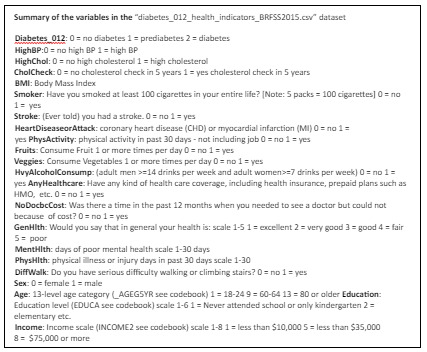
\includegraphics[width=3.125in,height=\textheight]{images/Captura de pantalla 2023-10-08 125457.jpg}
\caption{Characteristics of the data set variables}
\end{figure}

later using the function \texttt{psych} we can extract a statistical
analysis of the 22 variables contained in the dataset, which include the
mean, standard deviation, minimum and maximum range, among others.

Finally, using the \texttt{mutate} function we are going to transform
all the data that are not ``= 0'' in the variable Diabetes\_012, then we
will show in a small table how many data were classified as ``0'' or
``1'''' in this variable of our set of data

\begin{Shaded}
\begin{Highlighting}[]
\NormalTok{test\_diabetes}\OtherTok{\textless{}{-}}\NormalTok{ data\_set\_dia }\SpecialCharTok{\%\textgreater{}\%} \FunctionTok{mutate}\NormalTok{(}\AttributeTok{Diabetes\_012 =} \FunctionTok{ifelse}\NormalTok{(Diabetes\_012}\SpecialCharTok{!=} \StringTok{"0"}\NormalTok{, }\StringTok{"1"}\NormalTok{,Diabetes\_012))}
\end{Highlighting}
\end{Shaded}

\begin{Shaded}
\begin{Highlighting}[]
\NormalTok{Conteo\_Diabetes}
\end{Highlighting}
\end{Shaded}

\begin{verbatim}
## 
##      0      1 
## 213703  39977
\end{verbatim}

\hypertarget{part-2-knn}{%
\subsubsection{Part 2: KNN}\label{part-2-knn}}

In this part of the document we will use the KNN predictive method, for
this we will use 3 different variables to achieve the predictions.
First, through a stratified sample, we will take approximately 1\% of
the data to train our models.

\begin{Shaded}
\begin{Highlighting}[]
\NormalTok{ss\_diabetes }\OtherTok{\textless{}{-}}\NormalTok{ test\_diabetes }\SpecialCharTok{\%\textgreater{}\%}
  \FunctionTok{group\_by}\NormalTok{(Diabetes\_012) }\SpecialCharTok{\%\textgreater{}\%}
  \FunctionTok{sample\_n}\NormalTok{(}\DecValTok{1269}\NormalTok{, }\AttributeTok{replace =} \ConstantTok{TRUE}\NormalTok{) }\SpecialCharTok{\%\textgreater{}\%}
  \FunctionTok{ungroup}\NormalTok{()}
\end{Highlighting}
\end{Shaded}

\begin{Shaded}
\begin{Highlighting}[]
\NormalTok{Conteo\_ss\_Diabetes}
\end{Highlighting}
\end{Shaded}

\begin{verbatim}
## 
##    0    1 
## 1269 1269
\end{verbatim}

At this point we will find the appropriate number of ``K'' and we will
train the Knn model to predict Diabetes

\begin{Shaded}
\begin{Highlighting}[]
\FunctionTok{set.seed}\NormalTok{(}\DecValTok{123}\NormalTok{)  }
\NormalTok{indices }\OtherTok{\textless{}{-}} \FunctionTok{createFolds}\NormalTok{(ss\_diabetes}\SpecialCharTok{$}\NormalTok{Diabetes\_012, }\AttributeTok{k =} \DecValTok{10}\NormalTok{)}
\NormalTok{k\_values }\OtherTok{\textless{}{-}} \DecValTok{1}\SpecialCharTok{:}\DecValTok{20}
\NormalTok{resultados }\OtherTok{\textless{}{-}} \FunctionTok{data.frame}\NormalTok{(}\AttributeTok{K =}\NormalTok{ k\_values, }\AttributeTok{Error =} \FunctionTok{numeric}\NormalTok{(}\FunctionTok{length}\NormalTok{(k\_values)))}
\ControlFlowTok{for}\NormalTok{ (k }\ControlFlowTok{in}\NormalTok{ k\_values) \{}
\NormalTok{  errores }\OtherTok{\textless{}{-}} \FunctionTok{c}\NormalTok{()}

  \ControlFlowTok{for}\NormalTok{ (fold }\ControlFlowTok{in} \DecValTok{1}\SpecialCharTok{:}\DecValTok{10}\NormalTok{) \{}
\NormalTok{    train\_data\_ss\_diabetes }\OtherTok{\textless{}{-}}\NormalTok{ ss\_diabetes[}\SpecialCharTok{{-}}\NormalTok{indices[[fold]], ]}
\NormalTok{    test\_data\_ss\_diabetes }\OtherTok{\textless{}{-}}\NormalTok{ ss\_diabetes[indices[[fold]], ]}
    
\NormalTok{  prediction}\OtherTok{\textless{}{-}} \FunctionTok{knn}\NormalTok{(}\AttributeTok{train =}\NormalTok{ train\_data\_ss\_diabetes[, }\SpecialCharTok{{-}}\FunctionTok{ncol}\NormalTok{(train\_data\_ss\_diabetes)],}
                 \AttributeTok{test =}\NormalTok{ test\_data\_ss\_diabetes[,}\SpecialCharTok{{-}}\FunctionTok{ncol}\NormalTok{(test\_data\_ss\_diabetes)],}
                 \AttributeTok{cl =}\NormalTok{ train\_data\_ss\_diabetes}\SpecialCharTok{$}\NormalTok{Diabetes\_012, }
                  \AttributeTok{k =}\NormalTok{ k)}
\NormalTok{  error }\OtherTok{\textless{}{-}} \FunctionTok{mean}\NormalTok{(prediction }\SpecialCharTok{!=}\NormalTok{ test\_data\_ss\_diabetes}\SpecialCharTok{$}\NormalTok{Diabetes\_012)}
\NormalTok{    errores }\OtherTok{\textless{}{-}} \FunctionTok{c}\NormalTok{(errores, error)}
    
\NormalTok{  \}}
\NormalTok{  error\_promedio }\OtherTok{\textless{}{-}} \FunctionTok{mean}\NormalTok{(errores)}
\NormalTok{   resultados[k, }\StringTok{"Error"}\NormalTok{] }\OtherTok{\textless{}{-}}\NormalTok{ error\_promedio}
\NormalTok{\}}
\NormalTok{ mejor\_k }\OtherTok{\textless{}{-}}\NormalTok{ k\_values[}\FunctionTok{which.min}\NormalTok{(resultados}\SpecialCharTok{$}\NormalTok{Error)]}
 \FunctionTok{cat}\NormalTok{(}\StringTok{"El valor optimo de K es:"}\NormalTok{, mejor\_k, }\StringTok{"}\SpecialCharTok{\textbackslash{}n}\StringTok{"}\NormalTok{)}
\end{Highlighting}
\end{Shaded}

\begin{verbatim}
## El valor optimo de K es: 9
\end{verbatim}

\begin{Shaded}
\begin{Highlighting}[]
\NormalTok{ Prediction\_diabetes }\OtherTok{\textless{}{-}} \FunctionTok{knn}\NormalTok{(}\AttributeTok{train =}\NormalTok{ ss\_diabetes[, }\SpecialCharTok{{-}}\FunctionTok{ncol}\NormalTok{(ss\_diabetes)],}
                    \AttributeTok{test =}\NormalTok{ ss\_diabetes[, }\SpecialCharTok{{-}}\FunctionTok{ncol}\NormalTok{(ss\_diabetes)],}
                    \AttributeTok{cl =}\NormalTok{ ss\_diabetes}\SpecialCharTok{$}\NormalTok{Diabetes\_012,}
                    \AttributeTok{k =}\NormalTok{ mejor\_k)}
 \FunctionTok{CrossTable}\NormalTok{(}\AttributeTok{x =}\NormalTok{ ss\_diabetes}\SpecialCharTok{$}\NormalTok{Diabetes\_012, }\AttributeTok{y =}\NormalTok{ Prediction\_diabetes}
\NormalTok{           , }\AttributeTok{prop.chisq =}\NormalTok{ F)}
\end{Highlighting}
\end{Shaded}

\begin{verbatim}
## 
##  
##    Cell Contents
## |-------------------------|
## |                       N |
## |           N / Row Total |
## |           N / Col Total |
## |         N / Table Total |
## |-------------------------|
## 
##  
## Total Observations in Table:  2538 
## 
##  
##                          | Prediction_diabetes 
## ss_diabetes$Diabetes_012 |         0 |         1 | Row Total | 
## -------------------------|-----------|-----------|-----------|
##                        0 |      1019 |       250 |      1269 | 
##                          |     0.803 |     0.197 |     0.500 | 
##                          |     0.870 |     0.183 |           | 
##                          |     0.401 |     0.099 |           | 
## -------------------------|-----------|-----------|-----------|
##                        1 |       152 |      1117 |      1269 | 
##                          |     0.120 |     0.880 |     0.500 | 
##                          |     0.130 |     0.817 |           | 
##                          |     0.060 |     0.440 |           | 
## -------------------------|-----------|-----------|-----------|
##             Column Total |      1171 |      1367 |      2538 | 
##                          |     0.461 |     0.539 |           | 
## -------------------------|-----------|-----------|-----------|
## 
## 
\end{verbatim}

After training our knn model with all the variables from the data set, 5
of these variables were eliminated and the knn and caret model were
retrained to find the optimal value of ``k'', that is, we will have 16
predictor variables taking into account Note that we removed 5 and we
have a target variable.

\begin{Shaded}
\begin{Highlighting}[]
\NormalTok{ss\_diabetes\_5predictors }\OtherTok{\textless{}{-}}\NormalTok{ss\_diabetes }\SpecialCharTok{\%\textgreater{}\%}
  \FunctionTok{select}\NormalTok{(Diabetes\_012,HighBP,HighChol,CholCheck,BMI,Smoker,Stroke,HeartDiseaseorAttack,PhysActivity,Fruits,Veggies,HvyAlcoholConsump,GenHlth,DiffWalk,Sex,Age,Income)}
\end{Highlighting}
\end{Shaded}

After selecting the predictor variables we will repeat the same step to
train the model and find the appropriate value of ``k''

\begin{Shaded}
\begin{Highlighting}[]
\NormalTok{ Prediction\_diabetes5 }\OtherTok{\textless{}{-}} \FunctionTok{knn}\NormalTok{(}\AttributeTok{train =}\NormalTok{ ss\_diabetes\_5predictors[, }\SpecialCharTok{{-}}\FunctionTok{ncol}\NormalTok{(ss\_diabetes\_5predictors)],}
                    \AttributeTok{test =}\NormalTok{ ss\_diabetes\_5predictors[, }\SpecialCharTok{{-}}\FunctionTok{ncol}\NormalTok{(ss\_diabetes\_5predictors)],}
                    \AttributeTok{cl =}\NormalTok{ ss\_diabetes\_5predictors}\SpecialCharTok{$}\NormalTok{Diabetes\_012,}
                    \AttributeTok{k =} \DecValTok{5}\NormalTok{)}
\FunctionTok{CrossTable}\NormalTok{(}\AttributeTok{x =}\NormalTok{ ss\_diabetes\_5predictors}\SpecialCharTok{$}\NormalTok{Diabetes\_012, }\AttributeTok{y =}\NormalTok{ Prediction\_diabetes5}
\NormalTok{           , }\AttributeTok{prop.chisq =}\NormalTok{ F)}
\end{Highlighting}
\end{Shaded}

\begin{verbatim}
## 
##  
##    Cell Contents
## |-------------------------|
## |                       N |
## |           N / Row Total |
## |           N / Col Total |
## |         N / Table Total |
## |-------------------------|
## 
##  
## Total Observations in Table:  2538 
## 
##  
##                                      | Prediction_diabetes5 
## ss_diabetes_5predictors$Diabetes_012 |         0 |         1 | Row Total | 
## -------------------------------------|-----------|-----------|-----------|
##                                    0 |      1178 |        91 |      1269 | 
##                                      |     0.928 |     0.072 |     0.500 | 
##                                      |     0.932 |     0.071 |           | 
##                                      |     0.464 |     0.036 |           | 
## -------------------------------------|-----------|-----------|-----------|
##                                    1 |        86 |      1183 |      1269 | 
##                                      |     0.068 |     0.932 |     0.500 | 
##                                      |     0.068 |     0.929 |           | 
##                                      |     0.034 |     0.466 |           | 
## -------------------------------------|-----------|-----------|-----------|
##                         Column Total |      1264 |      1274 |      2538 | 
##                                      |     0.498 |     0.502 |           | 
## -------------------------------------|-----------|-----------|-----------|
## 
## 
\end{verbatim}

\begin{Shaded}
\begin{Highlighting}[]
\NormalTok{ss\_diabetes\_5predictors }\OtherTok{\textless{}{-}}\NormalTok{ss\_diabetes }\SpecialCharTok{\%\textgreater{}\%}
  \FunctionTok{select}\NormalTok{()}
\end{Highlighting}
\end{Shaded}

\hypertarget{including-plots}{%
\subsection{Including Plots}\label{including-plots}}

You can also embed plots, for example:

\includegraphics{Deliverable_2_files/figure-latex/pressure-1.pdf}

Note that the \texttt{echo\ =\ FALSE} parameter was added to the code
chunk to prevent printing of the R code that generated the plot.

\end{document}
